\begin{figure}[t]
  \centering
  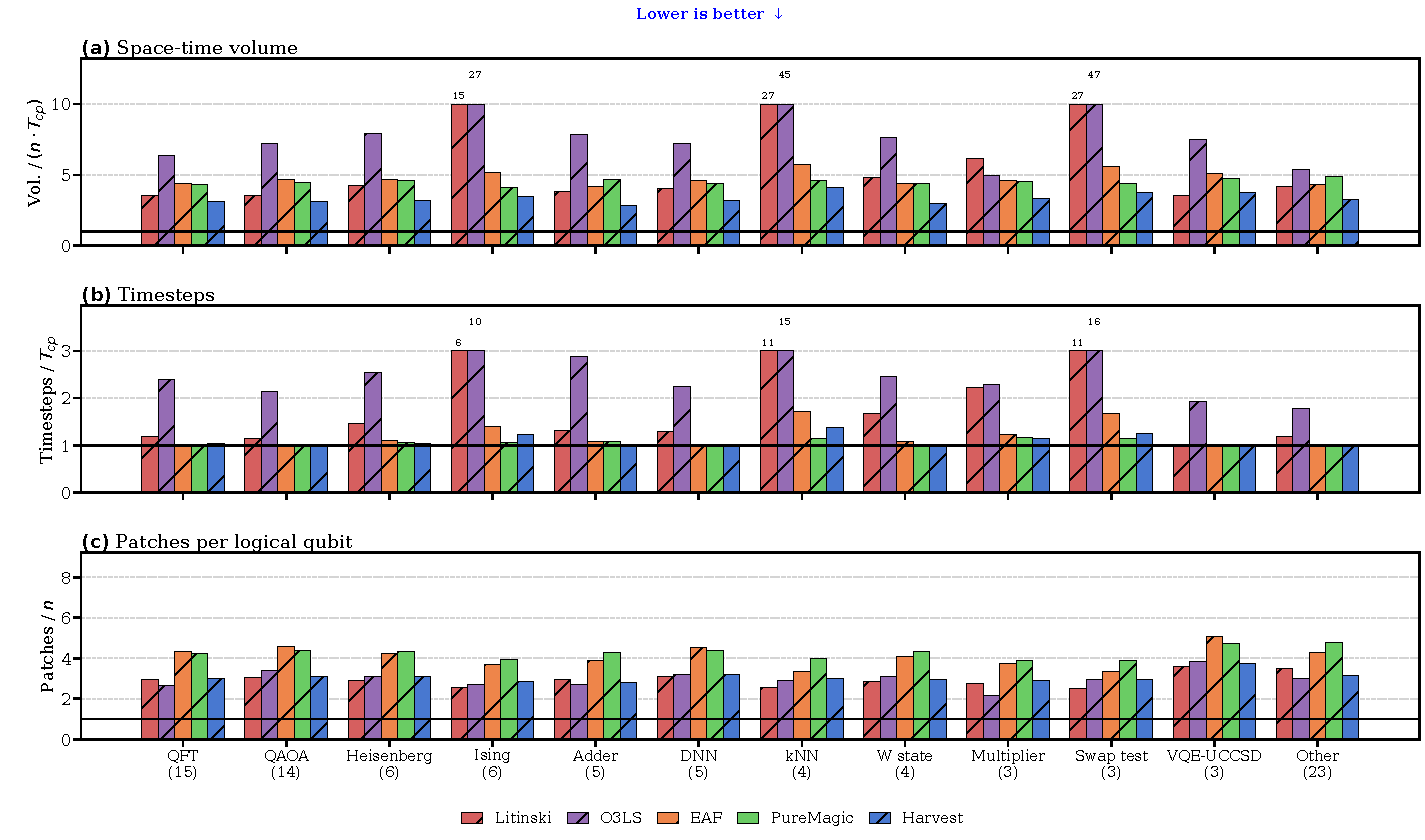
\includegraphics[width=\linewidth]{figures/evaluation/fig_rq1_family_instant.pdf}
  \caption{\textbf{Results per circuit family} (RQ1), instant magic states. Geometric means per family for \textbf{(a)}~normalized space--time volume, \textbf{(b)}~timesteps over the circuit depth, and \textbf{(c)}~patches per logical qubit. Families with fewer than three circuits are merged into \emph{Other}; numbers in parentheses give the circuits per family. The solid line marks the lower bound. Clipped bars are labeled with their value.}
  \label{fig:rq1-family-instant}
\end{figure}
